\section{Experiments and Results}
\label{sec:experiments}

\subsection{Setup}
\label{sec:methodology}

\paragraph{Base architecture.}
\looseness=-1 All experiments build on DreamerV3 \citep{hafner2025dreamerv3}, which learns an RSSM with discrete latent states ($32$ categories $\times$ $32$ classes), uses symlog-transformed predictions, and trains an actor-critic entirely in imagined trajectories. The default configuration imagines $H{=}15$ steps at $\dt{=}1$ (one imagination step per environment transition).

\paragraph{Variable-rate imagination.}
\label{sec:variable_rate}
\looseness=-1 We introduce three orthogonal modifications for variable-rate imagination.
\emph{Temporal embedding}: A learned embedding $e(\dt)$ is concatenated to the RSSM input at each imagination step; we test \textbf{trained} (backpropagation-updated), \textbf{frozen} (fixed random projection, \texttt{requires\_grad=False}), and \textbf{removed} ($d{=}0$).
\emph{Temporal subsampling}: The replay buffer augments training data with $\dt{>}1$ transitions by subsampling consecutive frames (max factor~2).
\emph{Horizon and step size}: $H \in \{15, 8\}$; \texttt{gate\_fixed\_dt} forces $\dt \in \{1, 2, 4\}$.

\paragraph{Factorial design.}
\label{sec:factorial}
\looseness=-1 We adopt a factorial ablation across four factors: $\dt$-embedding mode (trained / frozen / none), temporal subsampling (on / off), imagination horizon ($H{=}15$ / $H{=}8$), and step size ($\dt{=}1$, $2$, $4$). The design (12 conditions, Table~\ref{tab:factorial_design} in Appendix~\ref{sec:appendix_factorial}) isolates trained $\dt$-embedding and multi-rate exposure as orthogonal factors. Key configurations use 4--5 seeds; following \citet{agarwal2021precipice}, we report per-seed trajectories.

\paragraph{Diagnostic metric.}
\label{sec:metrics}
\looseness=-1 We define the normalized value-to-eval ratio $\nve_t = (v/e)_{\text{config},t} / (v/e)_{\text{baseline},t}$, where $v/e$ is the critic's mean imagined value divided by mean evaluation return, and the baseline is the highest-performing seed (exp\_001, seed~1, 505K steps). Analysis is restricted to a \textbf{35K+ window} to avoid early-training inflation. The $\nve \geq 2.0\times$ threshold classifies all $n{=}36$ configurations across two environments (AUROC${=}1.000$, F1${=}1.000$; Appendix~\ref{sec:appendix_sensitivity}); leave-one-environment-out cross-validation confirms robustness (Appendix~\ref{sec:nve_loeo}).

\paragraph{Intervention methods.}
\label{sec:sgs_method}
\looseness=-1 \emph{Selective gradient stopping} (SGS): $e_{\Delta t}$ is detached via $\operatorname{sg}(\cdot)$ before selected prediction heads during the backward pass. We test reward-only (exp\_016e), full-pathway (exp\_018), and obs-decoder-only (exp\_025/026) variants. \emph{Temporal conditioning noise} (TCN) adds Gaussian noise $\mathcal{N}(0, \sigma^2)$ to $e_{\Delta t}$ during imagination ($\sigma \in \{0.2, 0.5\}$, three environments); \emph{RAVE} clips imagined values exceeding an exponential moving average (EMA) anchor ($c \in \{2.0, 1.5\}$). \emph{Dual-critic}: a $2{\times}2$ factorial of \{single, dual\} $\times$ \{narrow (${\sim}1.2$M), wide (${\sim}2.4$M)\} critic following TD3 \citep{fujimoto2018td3}.
\label{sec:forward_pass_method}
\label{sec:dual_critic_method}

\paragraph{Environments and training.}
\label{sec:env_details}
\looseness=-1 All experiments use Walker Walk and Cheetah Run from the DeepMind Control Suite \citep{tassa2018dmcontrol} with proprioceptive observations. Walker Walk (6-joint biped) is the primary environment; Cheetah Run (6-joint runner) serves as a severity probe ($8$--$108\times$ NVE vs.\ $2$--$5\times$ on Walker). Baselines run 500K steps; treatments 105K steps. Hyperparameters follow DreamerV3 defaults \citep{hafner2025dreamerv3} (Appendix~\ref{sec:hyperparameters}); training uses a single GPU (${\sim}80$ GPU-hours total).

%% ============================================================
%% RESULTS
%% ============================================================

\subsection{F1: All Variable-Rate Configurations Degrade}
\label{sec:results}
\label{sec:f1}

\looseness=-1 Every configuration that introduces $\dt > 1$ imagination degrades relative to the $\dt{=}1$ baseline (Figure~\ref{fig:learning_curves}). The baseline reaches 915.7 at 105K; fixed $\dt{=}2$ (006) peaks at 485.3 before collapsing to 132.9 ($14\%$ of baseline); fixed $\dt{=}4$ (007) never exceeds 176.9 ($19\%$); the learned gate (005) collapses to just 98.8, representing $11\%$ of baseline performance.

\begin{figure}[t]
\centering
\begin{subfigure}[t]{0.49\columnwidth}
\centering
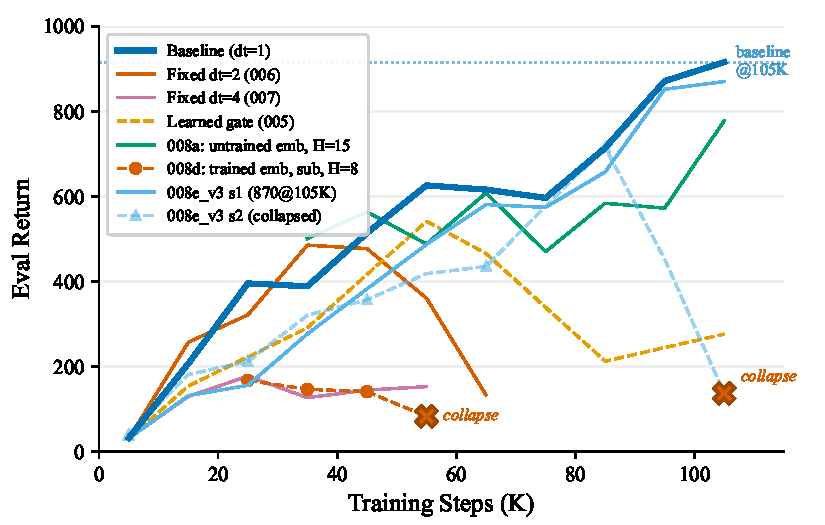
\includegraphics[width=\linewidth]{figures/paper/fig1_learning_curves.pdf}
\phantomcaption\label{fig:learning_curves}
\end{subfigure}\hfill
\begin{subfigure}[t]{0.49\columnwidth}
\centering
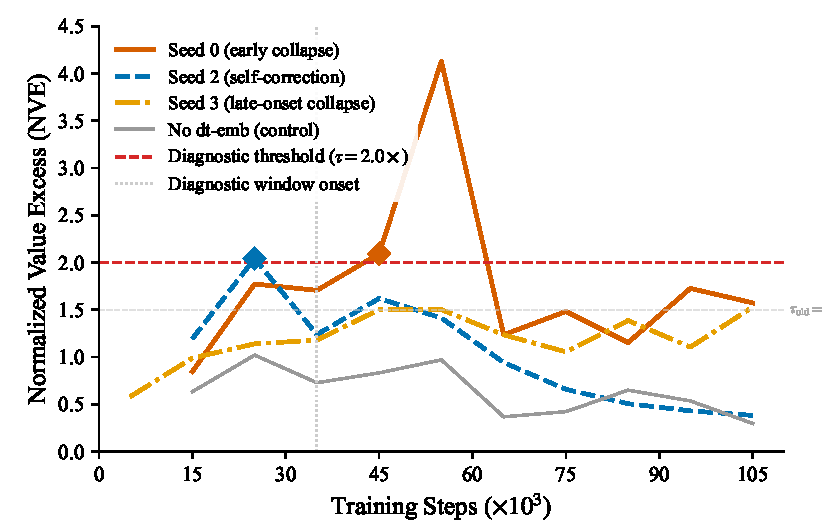
\includegraphics[width=\linewidth]{figures/fig1_nve_trajectory.pdf}
\phantomcaption\label{fig:nve_trajectory}
\end{subfigure}
\caption{(a) Variable-rate imagination universally degrades performance. Baseline (black) reaches 915.7; all variable-rate configs degrade. (b) NVE diagnostic separates CIVO-positive from healthy configurations: trained $\dt$-embedding seeds exceed the $2.0\times$ threshold; controls remain near $1.0\times$.}
\label{fig:curves_and_nve}
\end{figure}

%% ============================================================
%% TABLE 1: Main results summary
%% ============================================================

\begin{table*}[t]
\centering
\caption{Key configurations and outcomes. NVE reports peak $\nve$ in the 35K+ window (\S\ref{sec:metrics}). CIVO-positive seeds are shaded. Abbreviations: trn = trained ($d{=}32$, subsample ON); exp$^a$ = trained, subsample OFF; frz$^b$ = frozen ($d{=}32$, \texttt{requires\_grad=False}); --- = removed ($d{=}0$). $^c$~Environment-specific baseline. $^d$~Frozen control matches; environment-specific. $^e$~Seed-dependent (Table~\ref{tab:cross_domain}). $^f$~Corrected-code rerun (Appendix~\ref{sec:code_corrections}). $^g$~NVE median [range $0.31$--$127.6\times$]; mean$\pm$std dominated by outlier seed. Multi-seed entries report mean$\pm$std ($n$ noted in Config column). NVE reference baselines: Walker s1 (915.7); Cheetah $446.1$. Complete results for all 58 configurations in Table~\ref{tab:complete_results}.}
\label{tab:main_results}
\footnotesize
\setlength{\tabcolsep}{4pt}
\begin{tabular}{llcccccl}
\toprule
\textbf{Exp} & \textbf{Config} & \textbf{dt\_emb} & \textbf{Sub} & \textbf{H} & \textbf{Eval@final} & \textbf{NVE} & \textbf{Outcome} \\
\midrule
001 & Baseline ($\dt{=}1$, $n{=}4$) & --- & --- & 15 & $787.7 \pm 230.8$ & 1.00$\times$ & Healthy \\
\midrule
\rowcolor{gray!15}
008d & Factorial ($n{=}5$) & trn & ON & 8 & $190.6 \pm 90.2$ & $3.32 \pm 1.61\times$ & 3/5 onset \\
008f & No dt\_emb ($n{=}4$) & --- & ON & 8 & $302.4 \pm 134.8$ & $1.09 \pm 0.42\times$ & Healthy (0/4) \\
008a & Unexposed emb ($n{=}4$) & exp$^a$ & OFF & 15 & $820.9 \pm 68.8$ & $0.46 \pm 0.19\times$ & Healthy (0/4) \\
015b & Frozen emb & frz$^b$ & ON & 8 & 204.2 @105K & 1.45$\times$ & Grad.\ starvation \\
022b & Frozen emb + Gumbel gate & frz$^b$ & ON & 8 & 300.7 @105K & 0.63$\times$ & No CIVO \\
\midrule
\multicolumn{8}{l}{\textit{Cross-environment validation}} \\
\rowcolor{gray!15}
078 & Cheetah Run ($n{=}4$) & trn & ON & 8 & $123.2 \pm 132.9$ & med.\ $2.3\times$$^g$ & 3/4 onset \\
019b & PickCube-v1 & trn & ON & 8 & 26.64 @200K & 3.78$\times$$^c$ & Transient onset \\
049 & StackCube-v1 & trn & ON & 8 & 34.9 @212K & 5.05$\times$$^d$ & Env.\ transient \\
050 & PegInsertionSide-v1 & trn & ON & 8 & 20.86 @212K & 10.05$\times$$^e$ & Env.\ dynamics$^e$ \\
046 & Cheetah Run & frz$^b$ & ON & 8 & 150.5 @215K & 1.35$\times$ & No CIVO \\
\bottomrule
\end{tabular}
\end{table*}

%% ============================================================
%% F2: Trained dt_embedding → nve > 1.5x
%% ============================================================

\subsection{F2: Trained Temporal Embedding Precedes Value Overestimation}
\label{sec:f2}

\looseness=-1 The factorial design isolates trained $\dt$-embedding as the strongest predictor. The \emph{primary} comparison, 008d (trained, subsample ON) vs.\ 008f (no embedding, subsample ON), differs only in embedding training, yielding $\nve = 4.12\times$ (eval 82.8) vs.\ $\nve \leq 1.69\times$ (eval 139.5--468.8$^f$). \emph{Secondary} comparisons against 008a/008c (unexposed embedding) co-vary subsample status and horizon alongside the embedding factor. The $\nve \geq 2.0\times$ threshold (35K+ window) classifies all $n{=}36$ configurations across two environments (9 CIVO-positive, 27 non-CIVO; AUROC${=}1.000$, F1${=}1.000$; Table~\ref{tab:nve_loeo}; Figure~\ref{fig:nve_trajectory}).

\looseness=-1 The trained $\dt$-embedding triggers CIVO onset (NVE $\geq 2.0\times$) in 3 of 5 Walker Walk seeds, degrading all five to below 30\% of baseline (interquartile mean [IQM] $148.8$, $n{=}5$; \citet{agarwal2021precipice}). Including Cheetah Run (\S\ref{sec:f6}), CIVO onset occurs in 71\% of trained seeds (5/7; Clopper-Pearson 95\% CI: $[29\%, 96\%]$) versus 0/16 frozen or removed controls (Fisher exact $p < 0.001$); among onset cases, 3 sustain collapse, one self-corrects, one shows NVE self-correction without policy recovery (Appendix~\ref{sec:seed_divergence}).

\paragraph{Mechanism evidence.}
\looseness=-1 The RSSM reward head develops a $1.63\times$ prediction gap between $\dt{=}1$ and $\dt{=}2$ on Walker (Table~\ref{tab:rssm_fidelity}), but Cheetah shows no reward gap ($1.00\times$) despite higher CIVO severity ($8.27\times$); Cheetah observation fidelity reverses ($0.93\times$, $\dt{=}2$ predictions more accurate) while embedding geometry separates comparably (cosine ${\leq}{-}0.84$; Table~\ref{tab:cosine_sim}), indicating multiple transmission pathways. The critic internalizes the bias: mean $V(s)/\text{MC-return}$ reaches $7.80\times$ (100\% overestimated) vs.\ $1.05\times$ for the control. Evaluation return collapses ${\sim}35$K steps before actor entropy rises (Appendix~\ref{sec:civo_mechanism}).

\paragraph{Temporal ordering ($n{=}2$; correlational).}
\looseness=-1 Dense checkpoint analysis (12 points, 10K--65K) shows reward fidelity degradation precedes value overestimation: fidelity crosses $1.1\times$ at 20K while value-to-eval rises at ${\sim}$30K ($r{=}0.81$, $p{=}0.002$; Figure~\ref{fig:temporal_ordering}). A second seed confirms the pattern (lead ${\approx}$9K; Appendix~\ref{sec:timeseries_fidelity}). This temporal precedence is consistent with but does not establish a causal relationship.

\begin{figure}[t]
\centering
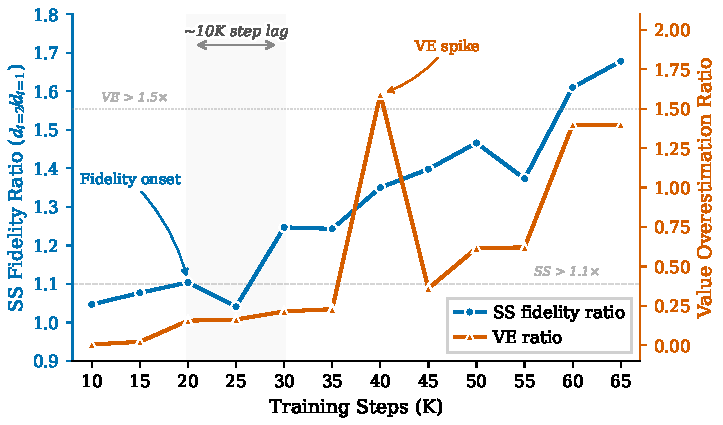
\includegraphics[width=0.75\columnwidth]{figures/paper/fig_temporal_ordering.pdf}
\caption{Temporal ordering of fidelity degradation and value overestimation (exp\_066, seed~0). \textbf{Left axis}: single-step fidelity ratio (blue) grows from $1.05\times$ to $1.68\times$. \textbf{Right axis}: value-to-eval ratio (red) remains near zero until 40K, then spikes. The ${\sim}$10K lag supports the causal direction: fidelity gap $\to$ value overestimation.}
\label{fig:temporal_ordering}
\end{figure}

%% ============================================================
%% F3--F5: Summary (details in Appendix B)
%% ============================================================

\subsection{F3--F5: Embedding Training Is a Necessary Causal Factor}
\label{sec:f3f5_summary}

\looseness=-1 Trained $\dt$-embedding triggers CIVO in 5/7 6-DoF locomotion seeds vs.\ 0/16 frozen or removed controls ($p < 0.001$; Table~\ref{tab:three_way_emb}); a random-policy decomposition attributes ${\approx}36\%$ of the effect to dynamics bias and ${\approx}64\%$ to actor exploitation (Appendix~\ref{sec:civo_mechanism}). Cross-environment validation on three ManiSkill \citep{gu2023maniskill2} tasks shows comparable value-ratio transients ($4$--$11\times$) with frozen controls matching, ruling out $\dt$-embedding causation (Table~\ref{tab:cross_domain}); CIVO is specific to moderate-complexity locomotion. The full factorial analysis appears in Appendix~\ref{sec:appendix_factorial}.

\looseness=-1 The gradient-condition analysis (Table~\ref{tab:three_way_emb}) reveals that no single pathway is responsible: reward-only detachment still produces CIVO (NVE $4.45\times$), and full-SGS partially mitigates one seed but fails to prevent collapse in the other. Only freezing or removing the embedding (0/10 seeds, NVE ${\leq}1.88\times$) eliminates CIVO, confirming gradient-driven co-adaptation as the root cause. The cross-environment boundary is equally informative: single-joint Cartpole Swingup produces 0/3 CIVO under the identical trigger configuration, and three ManiSkill manipulation tasks show comparable value-ratio transients ($4$--$11\times$) in both trained and frozen controls (Table~\ref{tab:cross_domain}). CIVO thus requires both a trained temporal embedding and multi-joint dynamics where temporal abstraction amplifies reward fidelity gaps.

\begin{table}[t]
\centering
\caption{$\dt$-embedding gradient conditions on Walker Walk. Any gradient pathway updating $e_{\dt}$ is sufficient to induce CIVO; freezing or removing the embedding dramatically reduces severity. $^*$Full-SGS seed~1 (NVE $1.66\times$); seed~2 collapsed. $^\dagger$Self-corrected at ${\sim}175$K (eval 44$\to$538, 59\% baseline).}
\label{tab:three_way_emb}
\footnotesize
\begin{tabular}{lccccl}
\toprule
Condition & Grad flow & Exp(s) & NVE peak & Eval & CIVO \\
\midrule
Trained & all & 008d, 059 & $1.53$--$4.72\times$ & 64--268 & 3/5 \\
Reward detach & obs+KL only & 044 & $4.45\times$ & 44$\to$538$^\dagger$ & 1/1 \\
Full SGS & KL only & 018 & $1.66\times$ & 448.3 & 1/1$^*$ \\
Frozen & none & 042, 015b, \ldots & $0.19$--$1.88\times$ & 124--612 & 0/6 \\
Removed & N/A & 008f & $0.76$--$1.69\times$ & 140--469 & 0/4 \\
\bottomrule
\end{tabular}
\end{table}

%% ============================================================
%% F6: dt=1 Imagination
%% ============================================================

\subsection{F6: $\dt{=}1$ Imagination Eliminates CIVO}
\label{sec:f6}

\looseness=-1 Restricting imagination to $\dt{=}1$ while retaining the trained embedding (exp\_008e\_v3; Appendix~\ref{sec:code_corrections}) yields 0/4 CIVO (peak NVE ${\leq}0.8\times$); three seeds achieve $65$--$96\%$ of baseline (mean $775.6$; Figure~\ref{fig:multiple_pathways}). The embedding still receives gradients, but the critic never encounters biased $\dt{>}1$ predictions. This localizes the vulnerability: the temporal embedding enables co-adaptation, but $\dt{>}1$ rollouts are required to propagate bias into the critic. While $\dt{=}1$ imagination eliminates CIVO, it also eliminates temporal abstraction, the original motivation for variable-rate imagination. The goal is not to avoid variable-rate imagination but to understand why it fails, so that future architectures can achieve temporal abstraction without triggering CIVO. The intervention analysis in \S\ref{sec:remedies} identifies the closed-loop structure of imagination as the fundamental barrier, directing future work toward architectures that decouple the critic's training distribution from the model that generates it.

\begin{figure}[t]
\centering
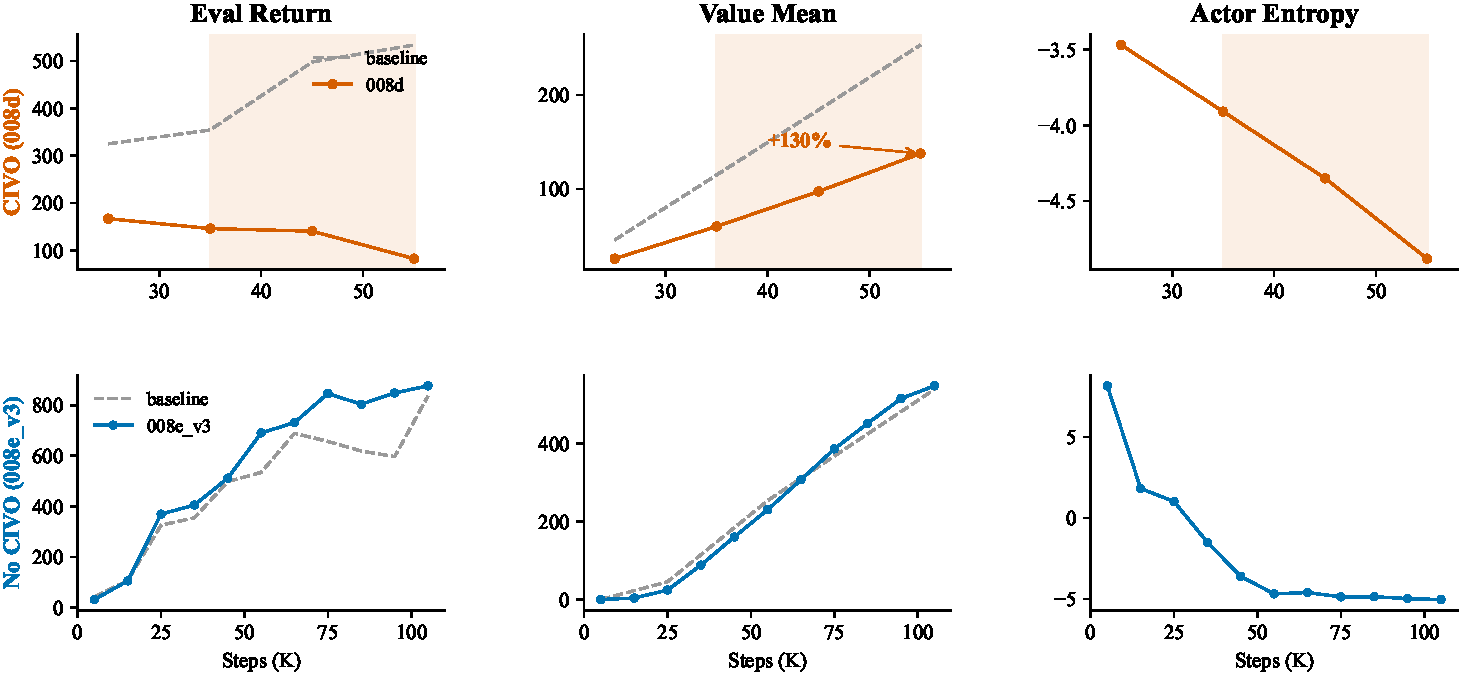
\includegraphics[width=\columnwidth]{figures/paper/fig6_multiple_pathways.pdf}
\caption{Contrasting dynamics ($2{\times}3$ grid). \textbf{Top row:} 008d (CIVO), showing eval collapse, value explosion, entropy decrease. \textbf{Bottom row:} 008e\_v3 s1 ($\dt{=}1$ imagination), no CIVO (NVE ${\leq}\,0.6\times$, eval $96\%$ baseline).}
\label{fig:multiple_pathways}
\end{figure}

